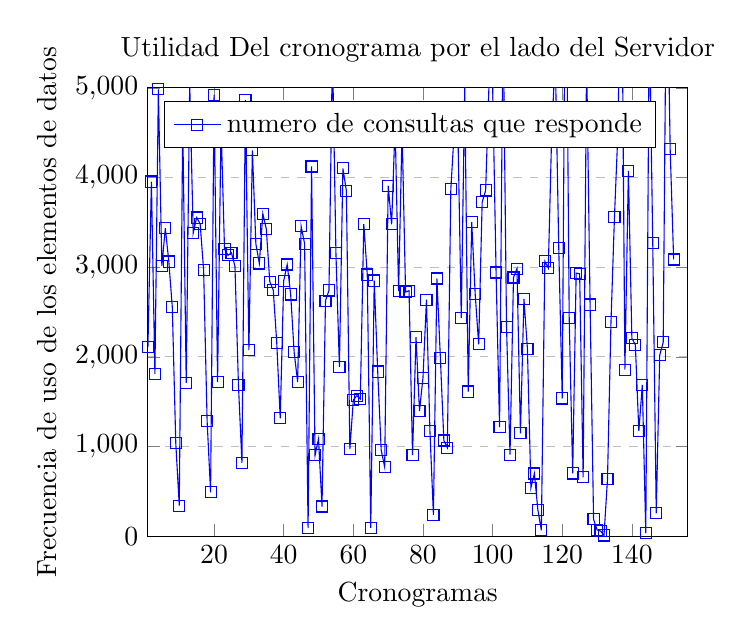
\begin{tikzpicture}
\begin{axis}[
    title={Utilidad Del cronograma por el lado del Servidor},
    xlabel={Cronogramas},
    ylabel={Frecuencia de uso de los elementos de datos},
    xmin=1, xmax=156,
    ymin=0, ymax=5000,
    xtick={},
    ytick={},
    legend pos=north west,
    ymajorgrids=true,
    grid style=dashed,
]

\addplot[
    color=blue,
    mark=square,
    ]
    coordinates {
%UTILIDAD TOTAL
%(cronograma, numero cues que usan al cronograma)
(1,2109)
(2,3955)
(3,1808)
(4,4983)
(5,3015)
(6,3434)
(7,3063)
(8,2554)
(9,1036)
(10,341)
(11,4608)
(12,1709)
(13,5051)
(14,3381)
(15,3554)
(16,3485)
(17,2966)
(18,1283)
(19,490)
(20,4925)
(21,1718)
(22,4587)
(23,3202)
(24,3133)
(25,3160)
(26,3009)
(27,1687)
(28,819)
(29,4863)
(30,2075)
(31,4303)
(32,3260)
(33,3042)
(34,3597)
(35,3426)
(36,2838)
(37,2745)
(38,2158)
(39,1314)
(40,2849)
(41,3030)
(42,2696)
(43,2050)
(44,1719)
(45,3457)
(46,3263)
(47,89)
(48,4123)
(49,902)
(50,1085)
(51,331)
(52,2627)
(53,2741)
(54,5430)
(55,3159)
(56,1888)
(57,4102)
(58,3853)
(59,968)
(60,1520)
(61,1567)
(62,1531)
(63,3480)
(64,2918)
(65,94)
(66,2851)
(67,1836)
(68,961)
(69,771)
(70,3910)
(71,3479)
(72,4593)
(73,2732)
(74,4536)
(75,2723)
(76,2738)
(77,904)
(78,2219)
(79,1396)
(80,1768)
(81,2637)
(82,1170)
(83,239)
(84,2874)
(85,1988)
(86,1067)
(87,988)
(88,3870)
(89,4530)
(90,4591)
(91,2436)
(92,5018)
(93,1613)
(94,3502)
(95,2698)
(96,2140)
(97,3725)
(98,3856)
(99,5081)
(100,5054)
(101,2941)
(102,1216)
(103,5863)
(104,2336)
(105,909)
(106,2885)
(107,2984)
(108,1147)
(109,2646)
(110,2092)
(111,540)
(112,699)
(113,295)
(114,65)
(115,3067)
(116,2990)
(117,4535)
(118,5339)
(119,3217)
(120,1536)
(121,7251)
(122,2435)
(123,700)
(124,2934)
(125,2927)
(126,656)
(127,5343)
(128,2583)
(129,189)
(130,70)
(131,57)
(132,8)
(133,638)
(134,2388)
(135,3562)
(136,4515)
(137,6964)
(138,1858)
(139,4075)
(140,2207)
(141,2135)
(142,1171)
(143,1688)
(144,33)
(145,5850)
(146,3270)
(147,255)
(148,2019)
(149,2162)
(150,6780)
(151,4319)
(152,3086)

    };
    \legend{numero de consultas que responde}

\end{axis}
\end{tikzpicture}

